
%% Nuclear Energy Questions used on the
%% NYSED Physics Regents Examination
%%--------------------------------------------------


%% this section contains 110 problems


%% Section June2014
%%--------------------
\element{nysed}{
\begin{question}{June2014-Q29}
    Which force is responsible for producing a stable nucleus by opposing the electrostatic force of repulsion between protons?
    \begin{multicols}{2}
    \begin{choices}
      \correctchoice{strong}
        \wrongchoice{frictional}
        \wrongchoice{weak}
        \wrongchoice{gravitational}
    \end{choices}
    \end{multicols}
\end{question}
}


%% NOTE: Jan2002 is the last exam to include Nuclear Energy


%% Section Jan2002
%%--------------------
\element{nysed}{
\begin{question}{Jan2002-Q106}
    If nitrogen nuclei are bombarded with alpha particles they can be changed into oxygen nuclei.
    This phenomenon is known as:
    \begin{choices}
        \wrongchoice{nuclear fission}
        \wrongchoice{nuclear fusion}
      \correctchoice{artificial transmutation}
        \wrongchoice{particle scattering}
    \end{choices}
\end{question}
}

\element{nysed}{
\begin{question}{Jan2002-Q107}
    One atomic mass unit is defined as:
    \begin{choices}
        \wrongchoice{the mass of an electron}
        \wrongchoice{the mass of an alpha particle}
        \wrongchoice{the mass of an atom of carbon-12}
      \correctchoice{\num{1/12} the mass of an atom of carbon-12}
    \end{choices}
\end{question}
}

\element{nysed}{
\begin{question}{Jan2002-Q108}
    According to the Uranium Disintegration Series,
        which nuclide is an isotope of lead (Pb)?
    \begin{multicols}{2}
    \begin{choices}
      \correctchoice{\ce{^{206}_{82}Pb}}
        \wrongchoice{\ce{^{214}_{88}Pb}}
        \wrongchoice{\ce{^{214}_{84}Pb}}
        \wrongchoice{\ce{^{222}_{86}Pb}}
    \end{choices}
    \end{multicols}
\end{question}
}

\element{nysed}{
\begin{question}{Jan2002-Q109}
    The nuclei of all the atoms in a single nuclide have:
    \begin{choices}
      \correctchoice{the same number of neutrons and the same number of protons}
        \wrongchoice{the same number of neutrons, but different numbers of protons}
        \wrongchoice{different numbers of neutrons, but the same number of protons}
        \wrongchoice{different numbers of neutrons and different numbers of protons}
    \end{choices}
\end{question}
}

\element{nysed}{
\begin{question}{Jan2002-Q110}
    What occurs when an atom emits gamma radiation?
    \begin{choices}
        \wrongchoice{The excited nucleus changes to a more stable state by absorbing a photon.}
      \correctchoice{The excited nucleus changes to a more stable state by emitting a photon.}
        \wrongchoice{The stable nucleus changes to an excited state by emitting a photon.}
        \wrongchoice{The stable nucleus changes to an excited state by absorbing a photon.}
    \end{choices}
\end{question}
}

\element{nysed}{
\begin{question}{Jan2002-Q111}
    What particle is represented by $X$ in the nuclear reaction
        \ce{^{9}_{4}Be + ^{4}_{2}He -> ^{12}_{6}C + $X$}?
    \begin{multicols}{4}
    \begin{choices}
        \wrongchoice{\ce{^{0}_{-1}e}}
        \wrongchoice{\ce{^{1}_{1}H}}
      \correctchoice{\ce{^{1}_{0}H}}
        \wrongchoice{\ce{^{2}_{1}H}}
    \end{choices}
    \end{multicols}
\end{question}
}

\element{nysed}{
\begin{question}{Jan2002-Q112}
    The half-life of a particular radioactive material is \SI{6.0}{\hour}.
    What fraction of a sample of the material would remain after \SI{1}{\day}?
    \begin{multicols}{4}
    \begin{choices}
        \wrongchoice{$\dfrac{1}{4}$}
        \wrongchoice{$\dfrac{2}{3}$}
        \wrongchoice{$\dfrac{3}{8}$}
      \correctchoice{$\dfrac{1}{16}$}
    \end{choices}
    \end{multicols}
\end{question}
}

\element{nysed}{
\begin{question}{Jan2002-Q113}
    Which device can be used to detect subatomic particles that exit nuclei?
    \begin{choices}
        \wrongchoice{Van de Graaff generator}
      \correctchoice{Geiger counter}
        \wrongchoice{linear accelerator}
        \wrongchoice{cyclotron}
    \end{choices}
\end{question}
}

\element{nysed}{
\begin{question}{Jan2002-Q114}
    In a nuclear reactor,
        which substance can be used as both the moderator and the coolant?
    \begin{multicols}{2}
    \begin{choices}
        \wrongchoice{cadmium}
        \wrongchoice{boron}
      \correctchoice{water}
        \wrongchoice{uranium}
    \end{choices}
    \end{multicols}
\end{question}
}

\element{nysed}{
\begin{question}{Jan2002-Q115}
    If the nucleus of an atom emits a positron,
        the atomic number of the atom will:
    \begin{multicols}{2}
    \begin{choices}
      \correctchoice{decrease by one}
        \wrongchoice{increase by one}
        \wrongchoice{remain unchanged}
        \wrongchoice{decrease by two}
    \end{choices}
    \end{multicols}
\end{question}
}


%% Section June2001
%%--------------------
\element{nysed}{
\begin{question}{June2001-Q106}
    Which nuclide has a mass number of 8?
    \begin{multicols}{4}
    \begin{choices}
        \wrongchoice{\ce{^{6}_{2}He}}
      \correctchoice{\ce{^{8}_{4}Be}}
        \wrongchoice{\ce{^{15}_{7}N}}
        \wrongchoice{\ce{^{16}_{8}O}}
    \end{choices}
    \end{multicols}
\end{question}
}

\element{nysed}{
\begin{question}{June2001-Q107}
    The binding energy of a uranium-235 nucleus is the energy equivalent of its:
    \begin{multicols}{2}
    \begin{choices}
        \wrongchoice{total mass}
        \wrongchoice{mass number}
        \wrongchoice{critical mass}
      \correctchoice{mass defect}
    \end{choices}
    \end{multicols}
\end{question}
}

\element{nysed}{
\begin{question}{June2001-Q108}
    Which device is used to detect nuclear radiation?
    \begin{choices}
        \wrongchoice{cyclotron}
      \correctchoice{Geiger counter}
        \wrongchoice{linear accelerator}
        \wrongchoice{Van de Graaff generator}
    \end{choices}
\end{question}
}

\element{nysed}{
\begin{question}{June2001-Q109}
    When an atom of \ce{^{238}_{92}U} decays to an atom of \ce{^{206}_{82}Pb},
        the total number of alpha particles emitted is Which device is used to detect nuclear radiation?
    \begin{multicols}{4}
    \begin{choices}
        \wrongchoice{5}
        \wrongchoice{6}
      \correctchoice{8}
        \wrongchoice{14}
    \end{choices}
    \end{multicols}
\end{question}
}

\element{nysed}{
\begin{question}{June2001-Q110}
    A medical lab has a \SI{16}{\gram} sample of a radioactive isotope.
    After \SI{6.0}{\hour},
        it is found that \SI{12}{\gram} of the sample have decayed.
    What is the half-life of the isotope?
    \begin{multicols}{2}
    \begin{choices}
        \wrongchoice{\SI{6.0}{\hour}}
        \wrongchoice{\SI{2.0}{\hour}}
      \correctchoice{\SI{3.0}{\hour}}
        \wrongchoice{\SI{12.0}{\hour}}
    \end{choices}
    \end{multicols}
\end{question}
}

\element{nysed}{
\begin{question}{June2001-Q111}
    The nuclear equation \ce{^{30}_{15}P -> ^{30}_{14}Si + ^{0}_{+1}e} represents:
    \begin{multicols}{2}
    \begin{choices}
        \wrongchoice{alpha bombardment}
        \wrongchoice{electron capture}
        \wrongchoice{neutron emission}
      \correctchoice{positron emission}
    \end{choices}
    \end{multicols}
\end{question}
}

\element{nysed}{
\begin{question}{June2001-Q112}
    In a nuclear reactor,
        one of the primary functions of the coolant is to:
    \begin{choices}
        \wrongchoice{promote overheating in the reactor core}
      \correctchoice{transfer thermal energy to a heat exchanger}
        \wrongchoice{adjust the number of neutrons}
        \wrongchoice{protect the reactor operators from radiation}
    \end{choices}
\end{question}
}

\element{nysed}{
\begin{question}{June2001-Q113}
    Protons and neutrons are composed of smaller particles called:
    \begin{multicols}{2}
    \begin{choices}
      \correctchoice{quarks}
        \wrongchoice{baryons}
        \wrongchoice{alpha particles}
        \wrongchoice{bosons}
    \end{choices}
    \end{multicols}
\end{question}
}

\element{nysed}{
\begin{question}{June2001-Q114}
    The equation below represents a fission reaction in a nuclear reactor.
    \begin{equation*}
        \ce{^{1}_{0}n + ^{235}_{92}U -> ^{141}_{56}Ba + ^{92}_{36}Kr + 3^{1}_{0}n + \text{energy}}
    \end{equation*}
    Which product of this reaction must be absorbed by other \ce{^{235}_{92}U} nuclei to sustain a chain reaction?
    \begin{multicols}{2}
    \begin{choices}
        \wrongchoice{\ce{^{141}_{56}Ba}}
        \wrongchoice{\ce{^{92}_{36}Kr}}
      \correctchoice{\ce{^{1}_{0}n}}
        \wrongchoice{energy}
    \end{choices}
    \end{multicols}
\end{question}
}

\element{nysed}{
\begin{question}{June2001-Q115}
    Which equation represents the process by which the Sun produces energy?
    \begin{choices}
      \correctchoice{\ce{^{3}_{1}H + ^{1}_{1}H -> ^{4}_{2}He + Q}}
        \wrongchoice{\ce{^{235}_{92}U + ^{1}_{0}n -> ^{138}_{56}Ba + ^{95}_{36}Kr + 3^{1}_{0}n + Q}}
        \wrongchoice{\ce{^{14}_{6}C -> ^{14}_{7}N + ^{0}_{-1}e + Q}}
        \wrongchoice{\ce{^{40}_{19}K + ^{0}_{-1}e -> ^{40}_{18}Ar + Q}}
    \end{choices}
\end{question}
}


%% Section Jan2000
%%--------------------
\element{nysed}{
\begin{question}{June2000-Q106}
    The diagram below shows a nuclear reactor designed
        to obtain energy in the form of heat from a nuclear fission reaction.
    \begin{center}
        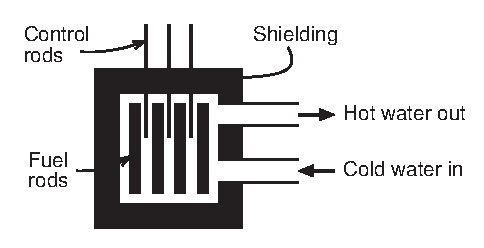
\includegraphics[keepaspectratio,scale=0.75]{Jan2001-Q106}
    \end{center}
    In the fission reaction
    \begin{equation*}
        ^{235}_{92}\mathrm{U}+^1_0\mathrm{n}\rightarrow F_1 + F_2 + 3^2_0\mathrm{n} + \mathrm{heat}
    \end{equation*}
    the fission fragments $F_1$ and $F_2$ might be:
    \begin{multicols}{2}
    \begin{choices}
      \correctchoice{$^{141}_{56}\mathrm{Ba}$ and $^{92}_{36}\mathrm{Kr}$}
        \wrongchoice{$^{141}_{56}\mathrm{Ba}$ and $^{93}_{36}\mathrm{Kr}$}
        \wrongchoice{$^{131}_{51}\mathrm{Sb}$ and $^{99}_{41}\mathrm{Nb}$}
        \wrongchoice{$^{132}_{51}\mathrm{Sb}$ and $^{99}_{41}\mathrm{Nb}$}
    \end{choices}
    \end{multicols}
\end{question}
}

\element{nysed}{
\begin{question}{June2000-Q107}
    The diagram below shows a nuclear reactor designed
        to obtain energy in the form of heat from a nuclear fission reaction.
    \begin{center}
        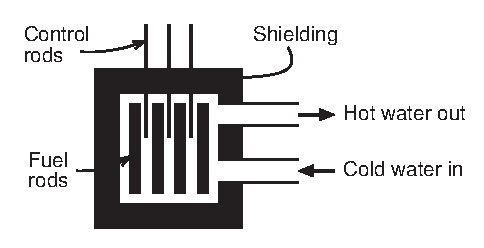
\includegraphics[keepaspectratio,scale=0.75]{Jan2001-Q106}
    \end{center}
    What is the total energy produced by converting
    \SI{1.0}{\kilo\gram} of $^{235}_{92}\mathrm{U}$ to energy in the reactor.
    \begin{multicols}{2}
    \begin{choices}
      \correctchoice{\SI{9.0e16}{\joule}}
        \wrongchoice{\SI{2.4e16}{\joule}}
        \wrongchoice{\SI{9.0e8}{\joule}}
        \wrongchoice{\SI{3.0e8}{\joule}}
    \end{choices}
    \end{multicols}
\end{question}
}

\element{nysed}{
\begin{question}{June2000-Q108}
    The diagram below shows a nuclear reactor designed
        to obtain energy in the form of heat from a nuclear fission reaction.
    \begin{center}
        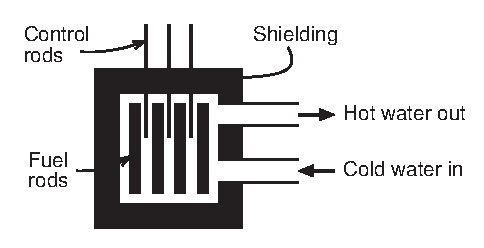
\includegraphics[keepaspectratio,scale=0.75]{Jan2001-Q106}
    \end{center}
    One of the radioactive waste products of the reactor has a half-life of \num{250} years.
    What fraction of a given sample of this product will remain after \num{1 000} years?
    \begin{multicols}{4}
    \begin{choices}
        \wrongchoice{$\dfrac{1}{2}$}
        \wrongchoice{$\dfrac{1}{4}$}
        \wrongchoice{$\dfrac{1}{8}$}
      \correctchoice{$\dfrac{1}{16}$}
    \end{choices}
    \end{multicols}
\end{question}
}

\element{nysed}{
\begin{question}{June2000-Q109}
    The diagram below shows a nuclear reactor designed
        to obtain energy in the form of heat from a nuclear fission reaction.
    \begin{center}
        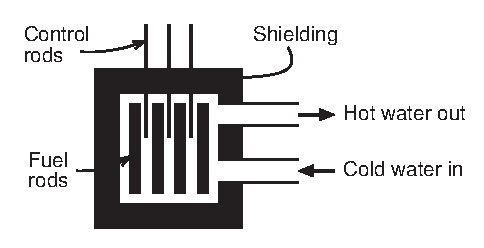
\includegraphics[keepaspectratio,scale=0.75]{Jan2001-Q106}
    \end{center}
    The water in the reactor acts both as a heat transfer agent and a moderator.
    In its capacity as a moderator, the water:
    \begin{choices}
        \wrongchoice{accelerates the neutrons to higher speeds so that they can interact with nuclei more energetically}
      \correctchoice{slows the neutrons to increase the probability of nuclear interaction}
        \wrongchoice{prevents a chain reaction from occurring}
        \wrongchoice{absorbs neutrons and slows the nuclear reaction}
    \end{choices}
\end{question}
}

\element{nysed}{
\begin{question}{June2000-Q110}
    The number of nucleons in a $^{206}_{82}\mathrm{Pb}$ nucleus is:
    \begin{multicols}{4}
    \begin{choices}
        \wrongchoice{\num{0}}
        \wrongchoice{\num{82}}
        \wrongchoice{\num{124}}
      \correctchoice{\num{206}}
    \end{choices}
    \end{multicols}
\end{question}
}

\element{nysed}{
\begin{question}{June2000-Q111}
    An atomic nucleus emits energy as it decays from an excited state
        to a more stable state without a change in its atomic number.
    This energy is emitted in the form of:
    \begin{multicols}{2}
    \begin{choices}
        \wrongchoice{an alpha particle}
      \correctchoice{an electron}
        \wrongchoice{a gamma ray}
        \wrongchoice{a beta particle}
    \end{choices}
    \end{multicols}
\end{question}
}

\element{nysed}{
\begin{question}{June2000-Q112}
    Which process occurs as nitrogen nuclei are bombarded by alpha particles to produce an isotope of oxygen?
    \begin{choices}
        \wrongchoice{photoelectric emission}
        \wrongchoice{thermionic emission}
        \wrongchoice{fission}
      \correctchoice{transmutation}
    \end{choices}
\end{question}
}

\element{nysed}{
\begin{question}{June2000-Q113}
    The particle $^{0}_{+1}\mathrm{e}$ is called a:
    \begin{multicols}{2}
    \begin{choices}
      \correctchoice{positron}
        \wrongchoice{proton}
        \wrongchoice{neutron}
        \wrongchoice{photon}
    \end{choices}
    \end{multicols}
\end{question}
}

\element{nysed}{
\begin{question}{June2000-Q114}
    High temperatures are required for controlled nuclear fusion because nuclei must overcome the forces of:
    \begin{choices}
        \wrongchoice{electrostatic attraction}
      \correctchoice{electrostatic repulsion}
        \wrongchoice{magnetic attraction}
        \wrongchoice{magnetic repulsion}
    \end{choices}
\end{question}
}

\element{nysed}{
\begin{question}{June2000-Q115}
    The nuclear force that holds nucleons together is:
    \begin{choices}
        \wrongchoice{weak and short range}
        \wrongchoice{weak and long range}
      \correctchoice{strong and short range}
        \wrongchoice{strong and long range}
    \end{choices}
\end{question}
}


%% Section June2000
%%--------------------
\element{nysed}{
\begin{question}{June2000-Q106}
    How much energy would be generated if a \SI{1.0e-3}{\kilo\gram} mass were completely converted to energy?
    \begin{multicols}{2}
    \begin{choices}
        \wrongchoice{\SI{9.3e-1}{\mega\eV}}
        \wrongchoice{\SI{9.3e2}{\mega\eV}}
      \correctchoice{\SI{9.0e13}{\joule}}
        \wrongchoice{\SI{9.0e16}{\joule}}
    \end{choices}
    \end{multicols}
\end{question}
}

\element{nysed}{
\begin{question}{June2000-Q107}
    One isotope of uranium is \ce{^{238}_{92}U}.
    Any other isotope of uranium must have:
    \begin{multicols}{2}
    \begin{choices}
      \correctchoice{92 protons}
        \wrongchoice{92 neutrons}
        \wrongchoice{146 protons}
        \wrongchoice{146 neutrons}
    \end{choices}
    \end{multicols}
\end{question}
}

\element{nysed}{
\begin{question}{June2000-Q108}
    A cyclotron is used in medical research to make radioisotopes.
    The primary function of a cyclotron is to
    \begin{choices}
        \wrongchoice{determine the mass of an atom}
        \wrongchoice{determine the half-life of a nuclide}
        \wrongchoice{accelerate neutrons}
      \correctchoice{accelerate charged particles}
    \end{choices}
\end{question}
}

\element{nysed}{
\begin{question}{June2000-Q109}
    As the nucleus of an unstable atom emits only gamma radiation,
        the nucleus must
    \begin{multicols}{2}
    \begin{choices}
        \wrongchoice{gain energy}
        \wrongchoice{lose protons}
      \correctchoice{lose energy}
        \wrongchoice{gain protons}
    \end{choices}
    \end{multicols}
\end{question}
}

\element{nysed}{
\begin{question}{June2000-Q110}
    In the reaction \ce{^{24}_{11}Na -> ^{24}_{12}Mg + $X$},
        the particle $X$ is a
    \begin{choices}
        \wrongchoice{positive electron}
      \correctchoice{negative electron}
        \wrongchoice{proton}
        \wrongchoice{neutron}
    \end{choices}
\end{question}
}

\element{nysed}{
\begin{question}{June2000-Q111}
    A \SI{24}{\gram} sample of a radioactive nuclide decayed
        to \SI{3.0}{\gram} of the nuclide in \SI{36}{\minute}.
    How much of the original nuclide sample remained
        after the first \SI{12}{\minute}?
    \begin{multicols}{2}
    \begin{choices}
      \correctchoice{\SI{12}{\gram}}
        \wrongchoice{\SI{6.0}{\gram}}
        \wrongchoice{\SI{2.0}{\gram}}
        \wrongchoice{\SI{8.0}{\gram}}
    \end{choices}
    \end{multicols}
\end{question}
}

\element{nysed}{
\begin{question}{June2000-Q112}
    A fusion reactor for commercial production of energy has not yet been developed.
    The best explanation for this situation is that fusion reactions
    \begin{choices}
        \wrongchoice{occur at extremely low temperatures}
        \wrongchoice{form highly radioactive products}
      \correctchoice{require very high energies}
        \wrongchoice{need fuels unavailable on Earth}
    \end{choices}
\end{question}
}

\element{nysed}{
\begin{question}{June2000-Q113}
    According to the Uranium Disintegration Series,
        how many beta particles are emitted when an
        \textsuperscript{206}\textsubscript{84}Po decays to
        \textsuperscript{206}\textsubscript{82}Pb.
    \begin{multicols}{4}
    \begin{choices}
        \wrongchoice{\num{7}}
        \wrongchoice{\num{6}}
        \wrongchoice{\num{3}}
      \correctchoice{\num{4}}
    \end{choices}
    \end{multicols}
\end{question}
}

\element{nysed}{
\begin{question}{June2000-Q114}
    In which nuclear equation does $X$ represent a neutron?
    \begin{choices}
        \wrongchoice{\ce{^{3}_{1}H + ^{1}_{1}H -> ^{4}_{2}H + $X$}}
        \wrongchoice{\ce{^{2}_{1}H + ^{2}_{1}H -> ^{3}_{1}H + ^{1}_{1}H + $X$}}
      \correctchoice{\ce{^{2}_{1}H + ^{3}_{1}H -> ^{4}_{2}He + $X$}}
        \wrongchoice{\ce{^{12}_{6}C + ^{1}_{0}n -> ^{13}_{7}N + $X$}}
    \end{choices}
\end{question}
}

\element{nysed}{
\begin{question}{June2000-Q115}
    Which statement best describes what occurs when the
        control rods are inserted into a nuclear reactor?
    \begin{choices}
      \correctchoice{The number of fission reactions decreases because the control rods absorb neutrons.}
        \wrongchoice{The number of fission reactions decreases because the control rods absorb electrons.}
        \wrongchoice{The number of fission reactions increases because the control rods release neutrons.}
        \wrongchoice{The number of fission reactions increases because the control rods release electrons.}
    \end{choices}
\end{question}
}


%% Section June1999
%%--------------------
\element{nysed}{
\begin{question}{June1999-Q106}
    Which type of force overcomes the repulsive electrostatic force
        between protons in the nucleus of an atom?
    \begin{multicols}{2}
    \begin{choices}
        \wrongchoice{magnetic}
      \correctchoice{nuclear}
        \wrongchoice{gravitational}
        \wrongchoice{centrifugal}
    \end{choices}
    \end{multicols}
\end{question}
}

\element{nysed}{
\begin{question}{June1999-Q107}
    The graph below represents the relationship between
        mass and its energy equivalent.
    \begin{center}
        \begin{tikzpicture}
            \begin{axis}[
                axis y line=left,
                axis x line=bottom,
                axis line style={->},
                xlabel={Mass},
                x unit=\si{\kilo\gram},
                xtick=\empty,
                ylabel={Energy},
                y unit=\si{\joule},
                ytick=\empty,
                xmin=0,xmax=11,
                ymin=0,ymax=11,
                grid=major,
                width=0.90\columnwidth,
                height=0.618\columnwidth,
                very thin,
            ]
            \addplot[line width=1pt,domain=0:10]{x};
            \end{axis}
        \end{tikzpicture}
    \end{center}
    The slope of the graph represents:
    \begin{choices}
        \wrongchoice{the electrostatic constant}
        \wrongchoice{gravitational field strength}
      \correctchoice{the speed of light squared}
        \wrongchoice{Planck's constant}
    \end{choices}
\end{question}
}

\element{nysed}{
\begin{question}{June1999-Q108}
    According to the Uranium Disintegration Series,
        an atom of uranium-238 changes to an atom of uranium-234 by the emission of:
    \begin{choices}
        \wrongchoice{one alpha particle followed by one beta particle}
        \wrongchoice{one beta particle followed by one alpha particle}
      \correctchoice{one alpha particle followed by two beta particle}
        \wrongchoice{one beta particle followed by two alpha particle}
    \end{choices}
\end{question}
}

\element{nysed}{
\begin{question}{June1999-Q109}
    An atom of \ce{^{131}_{53}I} and an atom of \ce{^{127}_{53}I} contain the same number of:
    \begin{multicols}{2}
    \begin{choices}
        \wrongchoice{quarks}
        \wrongchoice{neutrons}
        \wrongchoice{nucleons}
      \correctchoice{protons}
    \end{choices}
    \end{multicols}
\end{question}
}

\element{nysed}{
\begin{question}{June1999-Q110}
    The charge below lists the rest masses of two particles
        and a nucleus in atomic mass units.
    \begin{center}
    \begin{tabu}{X[r]X[l]}
        \toprule
        proton          & 1.0073u \\
        neutron         & 1.0087u \\
        \ce{^{6}_{3}Li} nucleus & 6.0135u \\
        \bottomrule
    \end{tabu}
    \end{center}
    What is the mass defect of a \ce{^{5}_{3}Li} nucleus?
    \begin{multicols}{2}
    \begin{choices}
      \correctchoice{\num{0.0345}u}
        \wrongchoice{\num{0.0615}u}
        \wrongchoice{\num{3.0606}u}
        \wrongchoice{\num{3.9975}u}
    \end{choices}
    \end{multicols}
\end{question}
}

\element{nysed}{
\begin{question}{June1999-Q111}
    The half-life of a radioactive nuclide is \SI{6}{\hour}.
    After one day (\SI{24}{\hour}), approximately how much of an original \SI{2.4e-2}{\kilo\gram} sample of this nuclide remains?
    \begin{multicols}{2}
    \begin{choices}
      \correctchoice{\SI{1.5e-3}{\kilo\gram}}
        \wrongchoice{\SI{2.4e-3}{\kilo\gram}}
        \wrongchoice{\SI{4.0e-3}{\kilo\gram}}
        \wrongchoice{\SI{6.0e-3}{\kilo\gram}}
    \end{choices}
    \end{multicols}
\end{question}
}

\element{nysed}{
\begin{question}{June1999-Q112}
    In the nuclear equation \ce{^{7}_{4}Be + $X$ -> ^{7}_{3}Li},
        $X$ represents:
    \begin{multicols}{2}
    \begin{choices}
        \wrongchoice{a proton}
        \wrongchoice{a positron}
        \wrongchoice{a neutron}
      \correctchoice{an electron}
    \end{choices}
    \end{multicols}
\end{question}
}

\element{nysed}{
\begin{question}{June1999-Q113}
    High-energy neutrons are released in all nuclear fission reactions.
    What material is used in a reactor to reduce the energy of these neutrons to thermal levels?
    \begin{multicols}{2}
    \begin{choices}
        \wrongchoice{shielding}
      \correctchoice{moderators}
        \wrongchoice{fissionable isotopes}
        \wrongchoice{thin metal foil}
    \end{choices}
    \end{multicols}
\end{question}
}

\element{nysed}{
\begin{question}{June1999-Q114}
    Which stable nucleus is formed when an unstable nucleus of \ce{^{137}_{56}Ba} emits a gamma ray?
    \begin{multicols}{2}
    \begin{choices}
      \correctchoice{\ce{^{137}_{56}Ba}}
        \wrongchoice{\ce{^{137}_{57}La}}
        \wrongchoice{\ce{^{138}_{55}Cs}}
        \wrongchoice{\ce{^{133}_{54}Xe}}
    \end{choices}
    \end{multicols}
\end{question}
}

\element{nysed}{
\begin{question}{June1999-Q115}
    The atomic mass unit is defined as \num{1/12} the mass of an atom of:
    \begin{multicols}{2}
    \begin{choices}
        \wrongchoice{\ce{^{8}_{4}Be}}
      \correctchoice{\ce{^{12}_{6}C}}
        \wrongchoice{\ce{^{22}_{11}Na}}
        \wrongchoice{\ce{^{24}_{12}Mg}}
    \end{choices}
    \end{multicols}
\end{question}
}


%% Section June1998
%%--------------------
\element{nysed}{
\begin{question}{June1998-Q106}
    The following is a nuclear decay path.
    \begin{equation*}
        \ce{^{32}_{16}S + ^{1}_{0}n -> ^{32}_{15}P + $X$}
    \end{equation*}
    How many neutrons are in an atom of \ce{^{32}_{15}P}?
    \begin{multicols}{4}
    \begin{choices}
        \wrongchoice{\num{15}}
        \wrongchoice{\num{16}}
      \correctchoice{\num{17}}
        \wrongchoice{\num{32}}
    \end{choices}
    \end{multicols}
\end{question}
}

\element{nysed}{
\begin{question}{June1998-Q107}
    The following is a nuclear decay path.
    \begin{equation*}
        \ce{^{32}_{16}S + ^{1}_{0}n -> ^{32}_{15}P + $X$}
    \end{equation*}
    What is particle $X$?
    \begin{multicols}{2}
    \begin{choices}
      \correctchoice{a proton}
        \wrongchoice{a neutron}
        \wrongchoice{an alpha particle}
        \wrongchoice{a beta particle}
    \end{choices}
    \end{multicols}
\end{question}
}

\element{nysed}{
\begin{question}{June1998-Q108}
    Compared to the gravitational force between two nucleons in an atom of helium,
        the nuclear force between the nucleons is:
    \begin{choices}
        \wrongchoice{weaker and has a shorter range}
        \wrongchoice{weaker and has a longer range}
      \correctchoice{stronger and has a shorter range}
        \wrongchoice{stronger and has a longer range}
    \end{choices}
\end{question}
}

\element{nysed}{
\begin{question}{June1998-Q109}
    The subatomic particles that make up protons are called:
    \begin{multicols}{2}
    \begin{choices}
        \wrongchoice{hyperons}
        \wrongchoice{baryons}
        \wrongchoice{positrons}
      \correctchoice{quarks}
    \end{choices}
    \end{multicols}
\end{question}
}

\element{nysed}{
\begin{question}{June1998-Q110}
    Which nuclear phenomenon produces a change in the mass number of a nucleus?
    \begin{multicols}{2}
    \begin{choices}
      \correctchoice{alpha decay}
        \wrongchoice{electron capture}
        \wrongchoice{gamma ray emission}
        \wrongchoice{positron emission}
    \end{choices}
    \end{multicols}
\end{question}
}

\element{nysed}{
\begin{question}{June1998-Q111}
    According to the Uranium Disintegration Series,
        how many different isotopes of polonium (Po) are formed as \ce{^{238}_{92}U} decays to \ce{^{206}_{82}Pb}?
    \begin{multicols}{4}
    \begin{choices}
        \wrongchoice{\num{1}}
        \wrongchoice{\num{2}}
        \wrongchoice{\num{3}}
        \wrongchoice{\num{0}}
    \end{choices}
    \end{multicols}
\end{question}
}

\element{nysed}{
\begin{question}{June1998-Q112}
    Gamma radiation consists of a stream of high-energy:
    \begin{multicols}{2}
    \begin{choices}
      \correctchoice{photons}
        \wrongchoice{protons}
        \wrongchoice{neutrons}
        \wrongchoice{electrons}
    \end{choices}
    \end{multicols}
\end{question}
}

\element{nysed}{
\begin{question}{June1998-Q113}
    A radioactive nuclide sample has a half-life of \SI{3.0}{\day}.
    If \SI{2.0}{\kilo\gram} of the sample remains unchanged after \SI{9.0}{\day},
        what was the initial mass of the sample?
    \begin{multicols}{2}
    \begin{choices}
        \wrongchoice{\SI{18}{\kilo\gram}}
      \correctchoice{\SI{16}{\kilo\gram}}
        \wrongchoice{\SI{8.0}{\kilo\gram}}
        \wrongchoice{\SI{6.0}{\kilo\gram}}
    \end{choices}
    \end{multicols}
\end{question}
}

\element{nysed}{
\begin{question}{June1998-Q114}
    Uranium-235 and plutonium-239 are used as fuels in nuclear reactors because of their:
    \begin{choices}
      \correctchoice{ability to undergo fission}
        \wrongchoice{ability to undergo fusion}
        \wrongchoice{inability to absorb neutrons}
        \wrongchoice{inability to release neutrons}
    \end{choices}
\end{question}
}

\element{nysed}{
\begin{question}{June1998-Q115}
    What is represented by the nuclear reaction below?
    \begin{equation*}
        \ce{^{2}_{1}H + ^{2}_{1}H -> ^{3}_{2}He + ^{1}_{0}n + energy}
    \end{equation*}
    \begin{multicols}{2}
    \begin{choices}
      \correctchoice{fusion}
        \wrongchoice{fission}
        \wrongchoice{alpha decay}
        \wrongchoice{beta decay}
    \end{choices}
    \end{multicols}
\end{question}
}


%% Section June1997
%%--------------------
\element{nysed}{
\begin{question}{June1997-Q106}
    In the transmutation reaction \ce{^{30}_{15}P -> $X$ + ^{0}_{+1}e},
        the $X$ represents:
    \begin{multicols}{2}
    \begin{choices}
        \wrongchoice{\ce{^{30}_{16}S}}
      \correctchoice{\ce{^{30}_{14}Si}}
        \wrongchoice{\ce{^{31}_{14}Si}}
        \wrongchoice{\ce{^{31}_{16}S}}
    \end{choices}
    \end{multicols}
\end{question}
}

\element{nysed}{
\begin{question}{June1997-Q107}
    What is the approximate binding energy of a helium nucleus that has a mass defect of \SI{5.2e-29}{\kilo\gram}?
    \begin{multicols}{2}
    \begin{choices}
        \wrongchoice{\SI{1.6e-21}{\joule}}
        \wrongchoice{\SI{1.6e-20}{\joule}}
        \wrongchoice{\SI{4.7e-13}{\joule}}
      \correctchoice{\SI{4.7e-12}{\joule}}
    \end{choices}
    \end{multicols}
\end{question}
}

\element{nysed}{
\begin{question}{June1997-Q108}
    Which pair correctly represents isotopes of the same element?
    \begin{multicols}{2}
    \begin{choices}
        \wrongchoice{\ce{^{210}_{82}Pb} and \ce{^{210}_{84}Po}}
        \wrongchoice{\ce{^{210}_{82}Pb} and \ce{^{210}_{84}Pb}}
      \correctchoice{\ce{^{210}_{82}Pb} and \ce{^{210}_{82}Pb}}
        \wrongchoice{\ce{^{210}_{84}Pb} and \ce{^{210}_{84}Po}}
    \end{choices}
    \end{multicols}
\end{question}
}

\element{nysed}{
\begin{question}{June1997-Q109}
    Which particle can \emph{not} be accelerated by a cyclotron?
    \begin{multicols}{2}
    \begin{choices}
        \wrongchoice{a proton}
      \correctchoice{a neutron}
        \wrongchoice{an alpha particle}
        \wrongchoice{an electron}
    \end{choices}
    \end{multicols}
\end{question}
}

\element{nysed}{
\begin{question}{June1997-Q110}
    According to the Uranium Disintegration Series,
        \ce{^{222}_{86}Rn} undergoes:
    \begin{choices}
      \correctchoice{an alpha decay, forming \ce{^{218}_{84}Po}}
        \wrongchoice{a beta decay, forming \ce{^{218}_{84}Po}}
        \wrongchoice{an alpha decay, forming \ce{^{226}_{88}Ra}}
        \wrongchoice{a beta decay, forming \ce{^{226}_{88}Ra}}
    \end{choices}
\end{question}
}

\element{nysed}{
\begin{question}{June1997-Q111}
    In the nuclear reaction represented below, what is particle $X$?
    \begin{equation*}
        \ce{^{238}_{93}Np -> ^{238}_{94}Pu + $X$}
    \end{equation*}
    \begin{multicols}{2}
    \begin{choices}
        \wrongchoice{a proton}
        \wrongchoice{a neutron}
      \correctchoice{an electron}
        \wrongchoice{a positron}
    \end{choices}
    \end{multicols}
\end{question}
}

\element{nysed}{
\begin{question}{June1997-Q112}
    A \SI{96}{\gram} sample of a radioactive nuclide is placed in a container.
    After \SI{12}{\minute},
        only \SI{6}{\gram} of the sample has not yet decayed.
    What is the half-life of the nuclide?
    \begin{multicols}{2}
    \begin{choices}
        \wrongchoice{\SI{6}{\minute}}
        \wrongchoice{\SI{2}{\minute}}
      \correctchoice{\SI{3}{\minute}}
        \wrongchoice{\SI{8}{\minute}}
    \end{choices}
    \end{multicols}
\end{question}
}

\element{nysed}{
\begin{question}{June1997-Q113}
    Which process is demonstrated by the reaction
    \begin{equation*}
        \ce{^{235}_{92}U + ^{1}_{0}n -> ^{141}_{56}Ba + ^{92}_{36}Kr + 3^{1}_{0}n + $Q$}\, ?
    \end{equation*}
    \begin{multicols}{2}
    \begin{choices}
      \correctchoice{nuclear fission}
        \wrongchoice{nuclear fusion}
        \wrongchoice{alpha decay}
        \wrongchoice{beta decay}
    \end{choices}
    \end{multicols}
\end{question}
}

\element{nysed}{
\begin{question}{June1997-Q114}
    The principle reason for using neutrons to bombard
        a nucleus is that neutrons:
    \begin{choices}
        \wrongchoice{have a relatively low atomic mass}
        \wrongchoice{have a very high kinetic energy}
        \wrongchoice{can be easily accelerated}
      \correctchoice{are not repelled by the nucleus}
    \end{choices}
\end{question}
}

\element{nysed}{
\begin{question}{June1997-Q115}
    Which process is the source of the Sun's energy?
    \begin{choices}
        \wrongchoice{natural radioactive decay}
        \wrongchoice{electron capture}
        \wrongchoice{fission}
      \correctchoice{fusion}
    \end{choices}
\end{question}
}


%% Section June1996
%%--------------------
\newcommand{\JuneOneNineNineSixQOneHundredSix}{
\begin{tabu}{X[r]X[l]}
    \toprule
    Particle & Rest Mass \\
    \midrule
    proton  & \SI{1.0073}{u} \\
    neutron & \SI{1.0087}{u} \\
    \bottomrule
\end{tabu}
}

\element{nysed}{
\begin{question}{June1996-Q106}
    The energy equivalent of the rest mass of a proton is approximately:
    \begin{center}
        \JuneOneNineNineSixQOneHundredSix
    \end{center}
    \begin{multicols}{2}
    \begin{choices}
        \wrongchoice{\SI{9.4e2}{\mega\eV}}
        \wrongchoice{\SI{1.9e3}{\mega\eV}}
        \wrongchoice{\SI{9.1e16}{\mega\eV}}
        \wrongchoice{\SI{6.4e18}{\mega\eV}}
    \end{choices}
    \end{multicols}
\end{question}
}

\element{nysed}{
\begin{question}{June1996-Q107}
    A tritium nucleus consists of one proton and two neutrons and has a total mass of \num{3.0170} atomic mass units.
    \begin{center}
        \JuneOneNineNineSixQOneHundredSix
    \end{center}
    What is the mass defect of the tritium nucleus?
    \begin{multicols}{2}
    \begin{choices}
        \wrongchoice{\SI{0.0014}{u}}
      \correctchoice{\SI{0.0077}{u}}
        \wrongchoice{\SI{1.0010}{u}}
        \wrongchoice{\SI{2.0160}{u}}
    \end{choices}
    \end{multicols}
\end{question}
}

\element{nysed}{
\begin{question}{June1996-Q108}
    Which force between the proton and neutrons in a tritium atom has the greatest magnitude?
    \begin{multicols}{2}
    \begin{choices}
        \wrongchoice{electrostatic force}
        \wrongchoice{gravitational force}
        \wrongchoice{magnetic force}
      \correctchoice{nuclear force}
    \end{choices}
    \end{multicols}
\end{question}
}

\element{nysed}{
\begin{question}{June1996-Q109}
    Tritium would most likely be used as a:
    \begin{choices}
        \wrongchoice{fuel in a fusion reaction}
      \correctchoice{fuel in a fission reaction}
        \wrongchoice{coolant in a nuclear reactor}
        \wrongchoice{moderator in a nuclear reactor}
    \end{choices}
\end{question}
}

\element{nysed}{
\begin{question}{June1996-Q110}
    A nuclear having an odd number of protons and an odd number of neutrons is likely to be radioactive.
    Which nuclide matches this description?
    \begin{multicols}{2}
    \begin{choices}
        \wrongchoice{\ce{^{29}_{14}Si}}
      \correctchoice{\ce{^{32}_{15}P}}
        \wrongchoice{\ce{^{32}_{16}S}}
        \wrongchoice{\ce{^{35}_{17}Cl}}
    \end{choices}
    \end{multicols}
\end{question}
}

\element{nysed}{
\begin{question}{June1996-Q111}
    How do cloud chambers, spark chambers,
        and Geiger counters aid in the study of the nucleus?
    \begin{choices}
      \correctchoice{They detect subatomic particles that exit the nucleus}
        \wrongchoice{They detect the presence of a magnetic field around the nucleus}
        \wrongchoice{They accelerate the nucleus before it collides with the particle beam}
        \wrongchoice{They accelerate subatomic particles that exit the nucleus}
    \end{choices}
\end{question}
}

\element{nysed}{
\begin{question}{June1996-Q112}
    Which nuclear particle is emitted as an atom of of \ce{^{238}_{92}U} decays to \ce{^{234}_{90}Th}?
    \begin{multicols}{2}
    \begin{choices}
        \wrongchoice{neutron}
        \wrongchoice{positron}
      \correctchoice{alpha particle}
        \wrongchoice{beta particle}
    \end{choices}
    \end{multicols}
\end{question}
}

\element{nysed}{
\begin{question}{June1996-Q113}
    In the equation below, what is particle $X$?
    \begin{equation*}
        \ce{^{9}_{4}Be + ^{4}_{2}He -> ^{12}_{6}C + X}
    \end{equation*}
    \begin{multicols}{2}
    \begin{choices}
        \wrongchoice{an electron}
        \wrongchoice{a proton}
        \wrongchoice{a positron}
      \correctchoice{a neutron}
    \end{choices}
    \end{multicols}
\end{question}
}

\element{nysed}{
\begin{question}{June1996-Q114}
    In a nuclear reactor,
        the function of a control rod is to:
    \begin{choices}
        \wrongchoice{slow down neutrons}
      \correctchoice{speed up neutrons}
        \wrongchoice{absorb neutrons}
        \wrongchoice{produce neutrons}
    \end{choices}
\end{question}
}

\element{nysed}{
\begin{question}{June1996-Q115}
    The radioactive waste strontium-90 has a half-life of 28 years.
    How long must a sample of strontium-90 be stored to insure that only $\frac{1}{16}$ of the original sample remains as radioactive strontium-90?
    \begin{multicols}{2}
    \begin{choices}
        \wrongchoice{28 years}
        \wrongchoice{56 years}
        \wrongchoice{84 years}
      \correctchoice{112 years}
    \end{choices}
    \end{multicols}
\end{question}
}


%% Section June1995
%%--------------------
\element{nysed}{
\begin{question}{June1995-Q49}
    Which observation was made by Rutherford when he bombarded gold foil with alpha particles?
    \begin{choices}
        \wrongchoice{Alpha particles were deflected toward a positive electrode}
      \correctchoice{Some alpha particles were deflected by the gold foil}
        \wrongchoice{Most alpha particles were scattered \ang{180} by the gold foil}
        \wrongchoice{Gold foil had no effect on the path of alpha particles}
    \end{choices}
\end{question}
}

\element{nysed}{
\begin{question}{June1995-Q106}
    Which atom has the same number of neutrons as \ce{^{16}_{8}O}?
    \begin{multicols}{2}
    \begin{choices}
        \wrongchoice{\ce{^{16}_{7}N}}
        \wrongchoice{\ce{^{17}_{8}O}}
      \correctchoice{\ce{^{15}_{7}N}}
        \wrongchoice{\ce{^{15}_{8}O}}
    \end{choices}
    \end{multicols}
\end{question}
}

\element{nysed}{
\begin{question}{June1995-Q107}
    The force that holds the nucleons of an atom together is:
    \begin{choices}
        \wrongchoice{weak and short-ranged}
        \wrongchoice{weak and long-ranged}
      \correctchoice{strong and short-ranged}
        \wrongchoice{strong and long-ranged}
    \end{choices}
\end{question}
}

\element{nysed}{
\begin{question}{June1995-Q108}
    Approximately how much energy is produced when 0.50 atomic mass unit of matter is completely converted into energy?
    \begin{multicols}{2}
    \begin{choices}
        \wrongchoice{\SI{9.3}{\mega\eV}}
        \wrongchoice{\SI{9.3e2}{\mega\eV}}
        \wrongchoice{\SI{4.7}{\mega\eV}}
      \correctchoice{\SI{4.7e2}{\mega\eV}}
    \end{choices}
    \end{multicols}
\end{question}
}

\element{nysed}{
\begin{question}{June1995-Q109}
    Atoms of different isotopes of the same element contain the same number of:
    \begin{choices}
        \wrongchoice{neutrons, but a different number of protons}
        \wrongchoice{neutrons, but a different number of electrons}
        \wrongchoice{electrons, but a different number of proton}
      \correctchoice{protons, but a different number of neutrons}
    \end{choices}
\end{question}
}

\element{nysed}{
\begin{question}{June1995-Q110}
    The disintegration of the nucleus of an atom of a naturally occurring radioactive element may produce more:
    \begin{choices}
        \wrongchoice{neutrons in the nucleus}
        \wrongchoice{electrons in the nucleus}
      \correctchoice{protons in the nucleus}
        \wrongchoice{atomic mass}
    \end{choices}
\end{question}
}

\element{nysed}{
\begin{question}{June1995-Q111}
    In the nuclear equation \ce{^{14}_{6}C -> ^{14}_{7}N + $X$}, the $X$ represents a:
    \begin{multicols}{2}
    \begin{choices}
      \correctchoice{beta particle}
        \wrongchoice{gamma ray}
        \wrongchoice{neutron}
        \wrongchoice{positron}
    \end{choices}
    \end{multicols}
\end{question}
}

\element{nysed}{
\begin{question}{June1995-Q112}
    The half-lift of a radium isotope is \num{1 600} years.
    After \num{4 800} years, approximately how much of the original \SI{10.0}{\kilo\gram} sample of the isotope will remain?
    \begin{multicols}{2}
    \begin{choices}
        \wrongchoice{\SI{0.125}{\kilo\gram}}
      \correctchoice{\SI{1.25}{\kilo\gram}}
        \wrongchoice{\SI{1.67}{\kilo\gram}}
        \wrongchoice{\SI{3.33}{\kilo\gram}}
    \end{choices}
    \end{multicols}
\end{question}
}

\element{nysed}{
\begin{question}{June1995-Q113}
    In nuclear reactors, neutrons are slowed down by:
    \begin{multicols}{2}
    \begin{choices}
      \correctchoice{moderators}
        \wrongchoice{control rods}
        \wrongchoice{fuel rods}
        \wrongchoice{accelerators}
    \end{choices}
    \end{multicols}
\end{question}
}

\element{nysed}{
\begin{question}{June1995-Q114}
    For nuclear fusion to occur,
        the reacting nucleus must:
    \begin{choices}
        \wrongchoice{absorb thermal neutrons}
      \correctchoice{have large kinetic energies}
        \wrongchoice{be fissionable}
        \wrongchoice{have a critical mass}
    \end{choices}
\end{question}
}

\element{nysed}{
\begin{question}{June1995-Q115}
    If the mass defect for nucleus $X$ is larger than the mass defect for nucleus $Y$,
        then nucleus $X$ has:
    \begin{choices}
        \wrongchoice{a smaller binding energy than nucleus $Y$}
      \correctchoice{a larger binding energy than nucleus $Y$}
        \wrongchoice{the same binding energy than nucleus $Y$}
    \end{choices}
\end{question}
}


%% Section June1994
%%--------------------
\element{nysed}{
\begin{question}{June1994-Q51}
    After Rutherford bombarded gold foil with alpha particles,
        he concluded that the volume of an atom is mostly empty space.
    Which observation led Rutherford to this conclusion?
    \begin{choices}
        \wrongchoice{Some of the alpha particles were deflected \ang{180}}
        \wrongchoice{The paths of the deflected alpha particles were hyperbolic}
        \wrongchoice{Many alpha particles were absorbed by gold nuclei}
      \correctchoice{Most of the alpha particles were not deflected}
    \end{choices}
\end{question}
}

\element{nysed}{
\begin{question}{June1994-Q106}
    How many neutrons are in an atom of \ce{^{222}_{86}Rn}?
    \begin{multicols}{4}
    \begin{choices}
        \wrongchoice{84}
        \wrongchoice{86}
      \correctchoice{136}
        \wrongchoice{222}
    \end{choices}
    \end{multicols}
\end{question}
}

\element{nysed}{
\begin{question}{June1994-Q107}
    The chart below shows the masses of selected particles.
    \begin{center}
    \renewcommand{\arraystretch}{1.5}
    \begin{tabu}{X[c]X[c]}
        \toprule
        Particle & Mass \\
        \midrule
        \ce{^{235}_{92}U} & 235.0 u \\
        \ce{^{138}_{56}Ba} & 137.9 u \\
        \ce{^{95}_{36}Kr} & 94.9 u \\
        \ce{^{1}_{0}n} & 1.0 u \\
        \bottomrule
    \end{tabu}
    \end{center}
    In the equation \ce{^{235}_{92}U + ^{1}_{0}n -> ^{138}_{56}Ba + ^{95}_{36}Kr + 3^{1}_{0}n + $E$},
        the energy $E$ is equivalent to a mass of:
    \begin{multicols}{2}
    \begin{choices}
      \correctchoice{0.2 u}
        \wrongchoice{2.0 u}
        \wrongchoice{2.2 u}
        \wrongchoice{0.0 u}
    \end{choices}
    \end{multicols}
\end{question}
}

\element{nysed}{
\begin{question}{June1994-Q108}
    Isotopes of the same element have nuclei with identical:
    \begin{choices}
        \wrongchoice{mass numbers}
        \wrongchoice{binding energies}
        \wrongchoice{number of neutrons}
      \correctchoice{number of protons}
    \end{choices}
\end{question}
}

\element{nysed}{
\begin{question}{June1994-Q109}
    Which subatomic particle can \emph{not} be accelerated by an electromagnetic field?
    \begin{multicols}{2}
    \begin{choices}
        \wrongchoice{alpha particle}
      \correctchoice{neutron}
        \wrongchoice{electron}
        \wrongchoice{positron}
    \end{choices}
    \end{multicols}
\end{question}
}

\element{nysed}{
\begin{question}{June1994-Q110}
    According to the Uranium Disintegration Series,
        the immediate decay produce of \ce{^{234}_{90}Th} is:
    \begin{multicols}{2}
    \begin{choices}
        \wrongchoice{\ce{^{230}_{92}U}}
        \wrongchoice{\ce{^{230}_{89}Ac}}
        \wrongchoice{\ce{^{238}_{92}U}}
      \correctchoice{\ce{^{234}_{91}Pa}}
    \end{choices}
    \end{multicols}
\end{question}
}

\element{nysed}{
\begin{question}{June1994-Q111}
    In the reaction \ce{^{27}_{13}Al + ^{4}_{2}He -> ^{30}_{15}P + ^{1}_{0}N + $X$},
        what could $X$ represent?
    \begin{multicols}{2}
    \begin{choices}
        \wrongchoice{proton}
      \correctchoice{gamma radiation}
        \wrongchoice{alpha particle}
        \wrongchoice{beta particle}
    \end{choices}
    \end{multicols}
\end{question}
}

\element{nysed}{
\begin{question}{June1994-Q112}
    A radioactive isotope has a half-life of 3 minutes.
    If \SI{19}{\kilo\gram} of this isotope remain after 15 minutes,
        the original mass of the isotope must have been:
    \begin{multicols}{2}
    \begin{choices}
        \wrongchoice{\SI{50}{\kilo\gram}}
        \wrongchoice{\SI{160}{\kilo\gram}}
        \wrongchoice{\SI{250}{\kilo\gram}}
      \correctchoice{\SI{320}{\kilo\gram}}
    \end{choices}
    \end{multicols}
\end{question}
}

\element{nysed}{
\begin{question}{June1994-Q113}
    When an atomic nucleus captures an electron,
        the atomic number of that nucleus:
    \begin{multicols}{2}
    \begin{choices}
      \correctchoice{decreases by 1}
        \wrongchoice{decreases by 2}
        \wrongchoice{increases by 1}
        \wrongchoice{increases by 1}
    \end{choices}
    \end{multicols}
\end{question}
}

\element{nysed}{
\begin{question}{June1994-Q114}
    The equation \ce{^{3}_{1}H + ^{1}_{1}H -> ^{4}_{2}He + energy} is an example of:
    \begin{multicols}{2}
    \begin{choices}
        \wrongchoice{alpha decay}
        \wrongchoice{positron capture}
      \correctchoice{fusion}
        \wrongchoice{fission}
    \end{choices}
    \end{multicols}
\end{question}
}

\element{nysed}{
\begin{question}{June1994-Q115}
    Which equation represents nuclear fission?
    \begin{choices}
        \wrongchoice{\ce{^{214}_{82}Pb -> ^{214}_{83}Bi + ^{0}_{-1}e}}
        \wrongchoice{\ce{4^{1}_{1}H -> ^{4}_{2}He + 2^{0}_{+1}e}}
      \correctchoice{\ce{^{235}_{92}U + ^{1}_{0}n -> ^{138}_{56}Ba + ^{95}_{36}Kr + 3^{1}_{0}n}}
        \wrongchoice{\ce{^{238}_{92}U -> ^{234}_{90}Th + ^{4}_{2}He}}
    \end{choices}
\end{question}
}


%% Section June1990
%%--------------------
\element{nysed}{
\begin{question}{June1990-Q111}
    Which nucleus has the greatest nuclear charge?
    \begin{multicols}{4}
    \begin{choices}
        \wrongchoice{\ce{^{2}_{1}W}}
      \correctchoice{\ce{^{8}_{5}X}}
        \wrongchoice{\ce{^{7}_{3}Y}}
        \wrongchoice{\ce{^{4}_{2}Z}}
    \end{choices}
    \end{multicols}
\end{question}
}

\element{nysed}{
\begin{question}{June1990-Q112}
    How much energy is released when \SI{1e-3}{\kilo\gram} of matter is converted to energy?
    \begin{multicols}{2}
    \begin{choices}
        \wrongchoice{\SI{3e5}{\joule}}
        \wrongchoice{\SI{3e8}{\joule}}
      \correctchoice{\SI{9e13}{\joule}}
        \wrongchoice{\SI{9e16}{\joule}}
    \end{choices}
    \end{multicols}
\end{question}
}

\element{nysed}{
\begin{question}{June1990-Q113}
    Which is an isotope of \ce{^{237}_{93}Np}?
    \begin{multicols}{2}
    \begin{choices}
        \wrongchoice{\ce{^{237}_{92}U}}
        \wrongchoice{\ce{^{237}_{94}Np}}
        \wrongchoice{\ce{^{235}_{92}U}}
      \correctchoice{\ce{^{235}_{93}Np}}
    \end{choices}
    \end{multicols}
\end{question}
}

\element{nysed}{
\begin{question}{June1990-Q114}
    Which force between the protons in a helium atom will have the greatest magnitude?
    \begin{choices}
        \wrongchoice{gravitational force}
        \wrongchoice{electrostatic force}
        %% also color force
      \correctchoice{nuclear force}
        \wrongchoice{magnetic force}
    \end{choices}
\end{question}
}

\element{nysed}{
\begin{question}{June1990-Q115}
    In the nuclear reaction \ce{^{218}_{84}Po -> ^{214}_{82}Pb + $X$}, the $X$ represents?
    \begin{multicols}{2}
    \begin{choices}
      \correctchoice{\ce{^{4}_{2}He}}
        \wrongchoice{\ce{^{0}_{-1}e}}
        \wrongchoice{\ce{^{0}_{+1}e}}
        \wrongchoice{\ce{^{1}_{0}n}}
    \end{choices}
    \end{multicols}
\end{question}
}

\element{nysed}{
\begin{question}{June1990-Q116}
    If a certain radioactive isotope has a half-life of 2 days,
        how much of a \SI{64}{\kilo\gram} sample of the isotope will remain after 10 days?
    \begin{multicols}{2}
    \begin{choices}
        \wrongchoice{\SI{1}{\kilo\gram}}
      \correctchoice{\SI{2}{\kilo\gram}}
        \wrongchoice{\SI{32}{\kilo\gram}}
        \wrongchoice{\SI{4}{\kilo\gram}}
    \end{choices}
    \end{multicols}
\end{question}
}

\element{nysed}{
\begin{question}{June1990-Q117}
    In the Uranium Disintegration Series,
        when an atom of \ce{^{238}_{92}U} decays to \ce{^{206}_{82}Pb},
        the total number of beta particles emitted is:
    \begin{multicols}{4}
    \begin{choices}
      \correctchoice{6}
        \wrongchoice{2}
        \wrongchoice{8}
        \wrongchoice{14}
    \end{choices}
    \end{multicols}
\end{question}
}

\element{nysed}{
\begin{question}{June1990-Q118}
    The equatoin \ce{^{27}_{13}Al + ^{4}_{2}He -> ^{30}_{15} + ^{1}_{0}n} is an example of:
    \begin{choices}
      \correctchoice{artificial transmutation}
        \wrongchoice{natural transmutation}
        \wrongchoice{alpha decay}
        \wrongchoice{beta decay}
    \end{choices}
\end{question}
}

\element{nysed}{
\begin{question}{June1990-Q119}
    Which part of a nuclear reactor would most likely contain plutonium?
    \begin{multicols}{2}
    \begin{choices}
        \wrongchoice{control rod}
      \correctchoice{fuel rod}
        \wrongchoice{moderator}
        \wrongchoice{shielding}
    \end{choices}
    \end{multicols}
\end{question}
}

\element{nysed}{
\begin{question}{June1990-Q120}
    Which statement best describes the fission products from nuclear reactors?
    \begin{choices}
        \wrongchoice{They are nonradioactive and may be safely discarded}
        \wrongchoice{They are nonradioactive and must be treated and/or stored}
        \wrongchoice{They are intensely radioactive and may be safely discarded}
      \correctchoice{They are intensely racioactive and must be treated and/or stored}
    \end{choices}
\end{question}
}


%% Section June1989
%%--------------------
\element{nysed}{
\begin{question}{June1989-Q111}
    What is the mass number of an atom with 9 protons, 11 neutrons, and 9 electrons?
    \begin{multicols}{4}
    \begin{choices}
        \wrongchoice{9}
        \wrongchoice{18}
      \correctchoice{20}
        \wrongchoice{29}
    \end{choices}
    \end{multicols}
\end{question}
}

\element{nysed}{
\begin{question}{June1989-Q112}
    If the mass of one proton is totally converted into energy,
        it will yield a total energy of:
    \begin{multicols}{2}
    \begin{choices}
        \wrongchoice{\SI{5.1e-19}{\joule}}
      \correctchoice{\SI{1.5e-10}{\joule}}
        \wrongchoice{\SI{9.3e8}{\joule}}
        \wrongchoice{\SI{9.0e16}{\joule}}
    \end{choices}
    \end{multicols}
\end{question}
}

\element{nysed}{
\begin{question}{June1989-Q113}
    The diagram below represents an inverted test tube over a sample of a radioactive material.
    Helium has collected in the test tube.
    \begin{center}
    \begin{tikzpicture}[font=\small]
        %% ground
        \draw (-1.5,0) -- (1.5,0);
        \node[anchor=north,minimum width=3cm,pattern=north east lines] at (0,0) {};
        %% test tube
        \draw (-0.5,0) -- (-0.5,2) arc (180:0:0.5) -- (0.5,0);
        \node[pin={[pin edge={latex-}]30:Helium}] at (0,2) {};
        \node[pin={[pin edge={latex-}]30:test tube}] at (0.5,1.25) {};
        %% sample
        \node[pin={[pin edge={latex-}]30:radioactive sample}] at (0.15,0.25) {};
        \draw[fill=white!60!black,domain=-0.5:0.5,smooth,samples=15] (-0.5,0) plot (\x, {0.33*exp(-6*\x*\x)*rnd}) -- (0.5,0) -- (-0.5,0);
    \end{tikzpicture}
    \end{center}
    The presence of helium indicates that the sample is most probably undergoing the process of:
    \begin{multicols}{2}
    \begin{choices}
      \correctchoice{alpha decay}
        \wrongchoice{beta decay}
        \wrongchoice{neutron decay}
        \wrongchoice{gamma emission}
    \end{choices}
    \end{multicols}
\end{question}
}

\element{nysed}{
\begin{question}{June1989-Q114}
    In the reaction \ce{^{24}_{11}Na -> ^{24}_{12}Mg + $x$}, what does $x$ represent?
    \begin{multicols}{2}
    \begin{choices}
        \wrongchoice{an alpha particle}
      \correctchoice{a beta particle}
        \wrongchoice{a neutron}
        \wrongchoice{a positron}
    \end{choices}
    \end{multicols}
\end{question}
}

\element{nysed}{
\begin{question}{June1989-Q115}
    The half-life of an isotope is 14 days.
    How many days will it take 8 grams of this isotope to decay to 1 gram?
    \begin{multicols}{4}
    \begin{choices}
        \wrongchoice{14}
        \wrongchoice{21}
        \wrongchoice{28}
      \correctchoice{42}
    \end{choices}
    \end{multicols}
\end{question}
}

\element{nysed}{
\begin{question}{June1989-Q116}
    The uranium isotope \ce{^{238}_{92}U} is used to produce:
    \begin{choices}
        \wrongchoice{shielding}
      \correctchoice{fissionable plutonium}
        \wrongchoice{control rods}
        \wrongchoice{heavy water}
    \end{choices}
\end{question}
}

\element{nysed}{
\begin{question}{June1989-Q117}
    Which reaction is an example of nuclear fission?
    \begin{choices}
        \wrongchoice{\ce{^{226}_{88}Ra -> ^{222}_{86}Rn + ^{4}_{2}He + Q}}
        \wrongchoice{\ce{^{214}_{83}Bi -> ^{214}_{84}Po + ^{0}_{-1}e + Q}}
        \wrongchoice{\ce{^{235}_{92}U + ^{1}_{0}n  -> ^{92}_{36}Kr + ^{141}_{56}Ba + 3^{1}_{0}n + Q}}
      \correctchoice{\ce{^{3}_{1}H + ^{1}_{1}H  -> ^{4}_{2}He + Q}}
    \end{choices}
\end{question}
}

\element{nysed}{
\begin{question}{June1989-Q118}
    The function of a moderator in a nuclear reactor is to:
    \begin{choices}
      \correctchoice{decrease the speed of the neutrons}
        \wrongchoice{increase the speed of the neutrons}
        \wrongchoice{decrease the number of the neutrons}
        \wrongchoice{increase the number of the neutrons}
    \end{choices}
\end{question}
}

\element{nysed}{
\begin{question}{June1989-Q119}
    Neutrons are used in some nuclear reactions as bombarding particles because they are:
    \begin{choices}
        \wrongchoice{positively charged and are repelled by the nucleus}
      \correctchoice{uncharged and are not repelled by the nucleus}
        \wrongchoice{negatively charged and are attracted by the nucleus}
        \wrongchoice{uncharged and have negligible mass}
    \end{choices}
\end{question}
}

\element{nysed}{
\begin{question}{June1989-Q120}
    When a nucleus captures an electron,
        the mass number of the nucleus:
    \begin{choices}
        \wrongchoice{decreases}
        \wrongchoice{increases}
      \correctchoice{remains the same}
    \end{choices}
\end{question}
}


%% Section June1986
%%--------------------
\element{nysed}{
\begin{question}{June1986-Q49}
    Rutherford observed that most of the alpha particles directed at a metallic foil appear to pass through unhindered,
        with only a few deflected at large angles.
    What did he conclude?
    \begin{choices}
        \wrongchoice{Alpha particles behave like waves when they interact with atoms.}
        \wrongchoice{Atoms have most of their mass distributed loosely in an electron cloud.}
        \wrongchoice{Atoms can easily absorb and reemit alpha particles.}
      \correctchoice{Atoms consist mainly of empty space and have small, dense nuclei.}
    \end{choices}
\end{question}
}

\element{nysed}{
\begin{question}{June1986-Q50}
    After the decay of a radioactive sample,
        helium gas was on the products.
    This suggests that the nuclear disintegration consisted of:
    \begin{multicols}{2}
    \begin{choices}
      \correctchoice{alpha particles}
        \wrongchoice{positron emissions}
        \wrongchoice{gamma emissions}
        \wrongchoice{beta decays}
    \end{choices}
    \end{multicols}
\end{question}
}

\element{nysed}{
\begin{question}{June1986-Q53}
    Isotopes of the same element must have different:
    \begin{multicols}{2}
    \begin{choices}
        \wrongchoice{numbers of protons}
        \wrongchoice{numbers of electrons}
        \wrongchoice{atomic numbers}
      \correctchoice{mass numbers}
    \end{choices}
    \end{multicols}
\end{question}
}

\element{nysed}{
\begin{question}{June1986-Q111}
    The equations represent a two-stage nuclear reaction.
    \begin{gather*}
        \ce{^{27}_{13}Al + ^{4}_{2}He -> ^{30}_{15}P + $X$} \\
        \ce{^{30}_{15}P -> ^{30}_{14}Si + $Y$ + energy}
    \end{gather*}
    Which nucleus in the two equations has the greatest number of neutrons?
    \begin{multicols}{2}
    \begin{choices}
        \wrongchoice{\ce{^{27}_{13}Al}}
        \wrongchoice{\ce{^{4}_{2}He}}
        \wrongchoice{\ce{^{30}_{15}P}}
      \correctchoice{\ce{^{30}_{14}Si}}
    \end{choices}
    \end{multicols}
\end{question}
}

\element{nysed}{
\begin{question}{June1986-Q112}
    The equations represent a two-stage nuclear reaction.
    \begin{gather*}
        \ce{^{27}_{13}Al + ^{4}_{2}He -> ^{30}_{15}P + $X$} \\
        \ce{^{30}_{15}P -> ^{30}_{14}Si + $Y$ + energy}
    \end{gather*}
    What is particle $X$?
    \begin{multicols}{2}
    \begin{choices}
        \wrongchoice{a positron}
        \wrongchoice{an electron}
        \wrongchoice{a proton}
      \correctchoice{a neutron}
    \end{choices}
    \end{multicols}
\end{question}
}

\element{nysed}{
\begin{question}{June1986-Q113}
    The equations represent a two-stage nuclear reaction.
    \begin{gather*}
        \ce{^{27}_{13}Al + ^{4}_{2}He -> ^{30}_{15}P + $X$} \\
        \ce{^{30}_{15}P -> ^{30}_{14}Si + $Y$ + energy}
    \end{gather*}
    Particle $Y$ represents?
    \begin{multicols}{2}
    \begin{choices}
        \wrongchoice{\ce{^{1}_{0}n}}
        \wrongchoice{\ce{^{1}_{1}H}}
      \correctchoice{\ce{^{0}_{+1}e}}
        \wrongchoice{\ce{^{0}_{-1}e}}
    \end{choices}
    \end{multicols}
\end{question}
}

\element{nysed}{
\begin{question}{June1986-Q114}
    Which graph best represents the relationship between energy and mass in the mass-energy equation?
    \begin{multicols}{2}
    \begin{choices}
        \AMCboxDimensions{down=-2.5em}
        %% ANS is 1
        \correctchoice{
            \begin{tikzpicture}
                \begin{axis}[
                    axis y line=left,
                    axis x line=bottom,
                    axis line style={->},
                    xlabel={mass},
                    xtick=\empty,
                    ylabel={energy},
                    ytick=\empty,
                    xmin=0,xmax=11,
                    ymin=0,ymax=11,
                    width=\columnwidth,
                    very thin,
                ]
                \addplot[line width=1pt,domain=0:10] {x};
                \end{axis}
            \end{tikzpicture}
        }
        \wrongchoice{
            \begin{tikzpicture}
                \begin{axis}[
                    axis y line=left,
                    axis x line=bottom,
                    axis line style={->},
                    xlabel={mass},
                    xtick=\empty,
                    ylabel={energy},
                    ytick=\empty,
                    xmin=0,xmax=11,
                    ymin=0,ymax=11,
                    width=\columnwidth,
                    very thin,
                ]
                \addplot[line width=1pt,domain=0:10] {0.1*x*x};
                \end{axis}
            \end{tikzpicture}
        }
        \wrongchoice{
            \begin{tikzpicture}
                \begin{axis}[
                    axis y line=left,
                    axis x line=bottom,
                    axis line style={->},
                    xlabel={mass},
                    xtick=\empty,
                    ylabel={energy},
                    ytick=\empty,
                    xmin=0,xmax=11,
                    ymin=0,ymax=11,
                    width=\columnwidth,
                    very thin,
                ]
                \addplot[line width=1pt,domain=0:10] {7};
                \end{axis}
            \end{tikzpicture}
        }
        \wrongchoice{
            \begin{tikzpicture}
                \begin{axis}[
                    axis y line=left,
                    axis x line=bottom,
                    axis line style={->},
                    xlabel={mass},
                    xtick=\empty,
                    ylabel={energy},
                    ytick=\empty,
                    xmin=0,xmax=11,
                    ymin=0,ymax=11,
                    width=\columnwidth,
                    very thin,
                ]
                \addplot[line width=1pt,domain=0:10] {10/x};
                \end{axis}
            \end{tikzpicture}
        }
    \end{choices}
    \end{multicols}
\end{question}
}

\element{nysed}{
\begin{question}{June1986-Q115}
    After two hours, \num{1/16} of the initial amount of radioactive isotope remains undecayed.
    What is the half-life of the isotope?
    \begin{multicols}{2}
    \begin{choices}
        \wrongchoice{\SI{15}{\minute}}
      \correctchoice{\SI{30}{\minute}}
        \wrongchoice{\SI{45}{\minute}}
        \wrongchoice{\SI{60}{\minute}}
    \end{choices}
    \end{multicols}
\end{question}
}

\element{nysed}{
\begin{question}{June1986-Q116}
    Neutrons are often used as bombarding particles in nuclear reactions because neutrons are:
    \begin{multicols}{2}
    \begin{choices}
        \wrongchoice{without mass}
        \wrongchoice{easy to accelerate}
      \correctchoice{electrically neutral}
        \wrongchoice{negatively charged}
    \end{choices}
    \end{multicols}
\end{question}
}

\element{nysed}{
\begin{question}{June1986-Q117}
    The functions of a moderator in a nuclear reactor is to:
    \begin{choices}
      \correctchoice{slow down neutrons}
        \wrongchoice{speed up neutrons}
        \wrongchoice{produce more neutrons}
        \wrongchoice{absorb neutrons}
    \end{choices}
\end{question}
}

\element{nysed}{
\begin{question}{June1986-Q118}
    During nuclear fusion,
        energy is released as a result of the:
    \begin{choices}
        \wrongchoice{splitting of heavy nuclei}
        \wrongchoice{combining of heavy nuclei}
      \correctchoice{combining of light nuclei}
        \wrongchoice{splitting of light nuclei}
    \end{choices}
\end{question}
}

\element{nysed}{
\begin{question}{June1986-Q119}
    When gamma radiation is emitted from a nucleus,
        the stability of the nucleus:
    \begin{choices}
        \wrongchoice{decreases}
      \correctchoice{increases}
        \wrongchoice{remains the same}
    \end{choices}
\end{question}
}

\element{nysed}{
\begin{question}{June1986-Q120}
    As metal foils of increasingly larger atomic number are bombarded by alpha particles,
        the number of alpha particles scatter beyond a given angle:
    \begin{choices}
        \wrongchoice{decreases}
      \correctchoice{increases}
        \wrongchoice{remains the same}
    \end{choices}
\end{question}
}


%% Section June1985
%%--------------------
\element{nysed}{
\begin{question}{June1985-Q31}
    Electromagnetic radiations are produced by:
    \begin{choices}
      \correctchoice{an accelerating alpha particle}
        \wrongchoice{an accelerating neutron}
        \wrongchoice{a proton at a constant velocity}
        \wrongchoice{an electron at a constant velocity}
    \end{choices}
\end{question}
}

\element{nysed}{
\begin{question}{June1985-Q32}
    Which particle has no charge?
    \begin{multicols}{2}
    \begin{choices}
        \wrongchoice{electron}
      \correctchoice{neutron}
        \wrongchoice{proton}
        \wrongchoice{alpha particle}
    \end{choices}
    \end{multicols}
\end{question}
}

\element{nysed}{
\begin{question}{June1985-Q52}
    A lithium nucleus contains three protons and four neutrons.
    What is its atomic mass number?
    \begin{multicols}{4}
    \begin{choices}
        \wrongchoice{1}
      \correctchoice{7}
        \wrongchoice{3}
        \wrongchoice{4}
    \end{choices}
    \end{multicols}
\end{question}
}

\element{nysed}{
\begin{question}{June1985-Q53}
    Which is an isotope of \ce{^{214}_{83}X}?
    \begin{multicols}{2}
    \begin{choices}
        \wrongchoice{\ce{^{214}_{82}X}}
        \wrongchoice{\ce{^{214}_{84}X}}
      \correctchoice{\ce{^{210}_{83}X}}
        \wrongchoice{\ce{^{210}_{82}X}}
    \end{choices}
    \end{multicols}
\end{question}
}

\element{nysed}{
\begin{question}{June1985-Q112}
    Which equation represents a fission reaction?
    The variables $x$ and $y$ represent unknown quantities.
    \begin{choices}
        \wrongchoice{\ce{^{230}_{90}Th ->  ^{214}_{82}Pb + $x$^{4}_{2}He}}
        \wrongchoice{\ce{^{14}_{7}N  ^{4}_{2}He  ->  ^{17}_{8}O + $y$}}
      \correctchoice{\ce{^{235}_{92}U + ^{1}_{0}n  ->  ^{90}_{38}Sr + ^{140}_{54}Xe + 6^{1}_{0}n }}
        \wrongchoice{\ce{^{3}_{1}H ^{1}_{1}H  ->  ^{4}_{2}He + energy}}
    \end{choices}
\end{question}
}

\element{nysed}{
\begin{question}{June1985-Q113}
    Which equation represents a part of the Uranium Disintegration Series?
    The variables $x$ and $y$ represent unknown quantities.
    \begin{choices}
      \correctchoice{\ce{^{230}_{90}Th ->  ^{214}_{82}Pb + $x$^{4}_{2}He}}
        \wrongchoice{\ce{^{14}_{7}N  ^{4}_{2}He  ->  ^{17}_{8}O + $y$}}
        \wrongchoice{\ce{^{235}_{92}U + ^{1}_{0}n  ->  ^{90}_{38}Sr + ^{140}_{54}Xe + 6^{1}_{0}n }}
        \wrongchoice{\ce{^{3}_{1}H ^{1}_{1}H  ->  ^{4}_{2}He + energy}}
    \end{choices}
\end{question}
}

\element{nysed}{
\begin{question}{June1985-Q114}
    In the following nuclear equation,
    \begin{displaymath}
        \ce{^{230}_{90}Th ->  ^{214}_{82}Pb + $x$^{4}_{2}He}
    \end{displaymath}
        what is the number of \ce{^{4}{2}He} particles represented by the coefficient $x$?
    \begin{multicols}{4}
    \begin{choices}
        \wrongchoice{1}
        \wrongchoice{2}
        \wrongchoice{3}
      \correctchoice{4}
    \end{choices}
    \end{multicols}
\end{question}
}

\element{nysed}{
\begin{question}{June1985-Q115}
    In the following nuclear equation,
    \begin{displaymath}
        \ce{^{14}_{7}N  ^{4}_{2}He  ->  ^{17}_{8}O + $y$}
    \end{displaymath}
        $y$ represents?
    \begin{multicols}{2}
    \begin{choices}
        \wrongchoice{a neutron}
        \wrongchoice{an electron}
      \correctchoice{a proton}
        \wrongchoice{an alpha particle}
    \end{choices}
    \end{multicols}
\end{question}
}

\element{nysed}{
\begin{question}{June1985-Q116}
    The number of neutrons in an atom of \ce{^{235}_{92}U} is:
    \begin{multicols}{4}
    \begin{choices}
        \wrongchoice{92}
      \correctchoice{143}
        \wrongchoice{235}
        \wrongchoice{327}
    \end{choices}
    \end{multicols}
\end{question}
}

\element{nysed}{
\begin{question}{June1985-Q117}
    In the following nuclear equation,
    \begin{displaymath}
        \ce{^{3}_{1}H ^{1}_{1}H  ->  ^{4}_{2}He + energy}
    \end{displaymath}
    compared to the nuclear mass of \ce{^{4}_{2}He},
        the sum of the nuclear masses of \ce{^{3}_{1}H} and \ce{^{1}_{1}H} is:
    \begin{multicols}{3}
    \begin{choices}
        \wrongchoice{less}
      \correctchoice{greater}
        \wrongchoice{the same}
    \end{choices}
    \end{multicols}
\end{question}
}

\element{nysed}{
\begin{question}{June1985-Q118}
    A pure sample of radon (Rn) gas is sealed inside a glass tube.
    The half-life of radon is 4 days.
    %% start question
    If the pressure inside the tube were decreased to one-half,
        the half-life of the radon would be:
    \begin{choices}
      \correctchoice{unchanged}
        \wrongchoice{doubled}
        \wrongchoice{decreased to one-half}
        \wrongchoice{decreased to one-quarter}
    \end{choices}
\end{question}
}

\element{nysed}{
\begin{question}{June1985-Q119}
    A pure sample of radon (Rn) gas is sealed inside a glass tube.
    The half-life of radon is 4 days.
    %% start question
    Twenty days after the radon was sealed inside the tube,
        the fraction of radon gas remaining would be:
    \begin{multicols}{4}
    \begin{choices}
        \wrongchoice{\num{1/2}}
        \wrongchoice{\num{1/8}}
        \wrongchoice{\num{1/16}}
      \correctchoice{\num{1/32}}
    \end{choices}
    \end{multicols}
\end{question}
}

\element{nysed}{
\begin{question}{June1985-Q120}
    A pure sample of radon (Rn) gas is sealed inside a glass tube.
    The half-life of radon is 4 days.
    %% start questoin
    The contents of the tube were analyzed after twenty days and another gas was found in addition to radon.
    This new gas is most likely:
    \begin{multicols}{2}
    \begin{choices}
      \correctchoice{helium}
        \wrongchoice{hydrogen}
        \wrongchoice{nitrogen}
        \wrongchoice{oxygen}
    \end{choices}
    \end{multicols}
\end{question}
}


\endinput


